
\section{Vire messages and JSON formatting}\label{app:json_fmt}

Within Vire  and between Vire  components and external  components, we
use  a communication  system based  on JSON-formatted  messages.  This
section describes the structure and the formatting of such messages.

\subsection{General structure of a message}

Each message consists in two parts (figure \ref{fig-app-json-message}):
\begin{itemize}

\item  the \emph{header}  is dedicated  to generic  informations which
  document the message itself.

\item  the \emph{body}  of the  message  contains the  real data.  Its
  encoding/decoding depends on the format specified in the header.

\end{itemize}

\begin{figure}[h]
\vskip 10pt
\small
\begin{Verbatim}[frame=single,xleftmargin=0.cm,label=\fbox{C++}]
struct message {
  msg_header header; // Header of the message
  msg_body   body;   // Body of the message
};
\end{Verbatim}
\normalsize
\caption{The structure of a message object (C++).}\label{fig-app-json-message}
\end{figure}

\subsection{The message header}

The header contains (figure \ref{fig-app-json-header}):
\begin{itemize}

  \item The mandatory \texttt{message\_id}  key contains an identifier
    of the  message which  document the emitter  and a  unique message
    number.   Each emitter  is  responsible of  the  numbering of  the
    messages it  emits, typically using an  incremental technique. The
    message  number is  a positive  integer, starting  from 0  (figure
    \ref{fig-app-json-message_id}).

  \item  The \texttt{format\_id}  key contains  the identifier  of the
    format  used  to encode  the  body  section.   It is  a  mandatory
    character  string.  The  default format  for message  transmission
    inside the  Vire API is \texttt{"vire::message::format::basic"} version
    \texttt{"1.0"} (figure \ref{fig-app-json-format_id}).

  \item The  \texttt{timestamp} key  contains a character  string that
    documents  the  approximative  time  point when  the  message  was
    created.       It       uses      the       following      format:
    \texttt{yyyymmddThhmmss.uuuuuu} where:

    \vskip -10pt
    \begin{itemize}
    \item[\texttt{yyyymmdd} :] encodes year/month/day,
    \item[\texttt{hhmmssd} :] encodes hour/minute/second,
    \item[\texttt{uuuuuu} :] encodes microseconds.
    \end{itemize}

  \item   In   the   case    of   a   \emph{response}   message,   the
    \texttt{in\_reply\_to} attribute is set to identify the associated
    request message.

\end{itemize}


\begin{figure}[h]
\vskip 10pt
\small
\begin{Verbatim}[frame=single,xleftmargin=0.cm,label=\fbox{C++}]
struct msg_header {
  message_identifier message_id;  // Message identifier from the emitter.
  format_identifier  format_id;   // Format identifier.
  std::string        timestamp;   // Timestamp.
  message_identifier in_reply_to; // Message identifier of the associated request message.
};
\end{Verbatim}
\normalsize
\caption{The  structure  of  a   message  header  object  (C++  class:
  \texttt{vire::message::msg\_header}).}\label{fig-app-json-header}
\end{figure}

\begin{figure}[h]
\vskip 10pt
\small
\begin{Verbatim}[frame=single,xleftmargin=0.cm,label=\fbox{C++}]
struct message_identifier {
  std::string emitter; // Name identifying the emitter of the message.
  int32_t     number;  // Number identifying the message in the emitter's
                       // message numbering scheme.
};
\end{Verbatim}
\normalsize
\caption{The      structure      of     a      message      identifier
  (C++).}\label{fig-app-json-message_id}
\end{figure}

\begin{figure}[h]
\vskip 10pt
\small
\begin{Verbatim}[frame=single,xleftmargin=0.cm,label=\fbox{C++}]
struct format_identifier {
  std::string name;    // Name identifying the format of the message.
  std::string version; // String identifying the version of the format.
};
\end{Verbatim}
\normalsize
\caption{The structure of a message format identifier (C++).}\label{fig-app-json-format_id}
\end{figure}


\begin{figure}[h]
\vskip 10pt
\small
\begin{Verbatim}[frame=single,xleftmargin=0.cm,label=\fbox{\texttt{JSON}}]
  {
    "header" : {
      "message_id" : {
        "emitter" : "vire.server",
        "number"  : "723"
      },
      "format_id"  : {
        "name" : "vire::message::format::basic",
        "version" : "1.0"
      },
      "timestamp" : "20160516T085346",
      "in_reply_to" : {
        "emitter" : "vire.client",
        "number"  : "843"
      }
    },
    "body" : {
      ... special layout for the payload data ...
    }
  }
\end{Verbatim}
\normalsize
\caption{Example    of    the    header   of    a    JSON    formatted
  message.}\label{fig-app-json-example-message}
\end{figure}

%% Timestamp string encoding

\clearpage

\subsection{The message body}

The     default     message     format    in     Vire     is     named
\texttt{"vire::message::format::basic"}    (version   \texttt{"1.0"}).
Each message  used within the Vire  framework is supposed to  use this
format.  The  general idea is that  the body of the  message encodes a
\emph{payload  object}   that  has  to  be   transmitted  between  two
components of  the system.   \emph{Payload objects} are  classified in
one of three categories:

\begin{enumerate}

\item Request : describes a request submitted by one component to another component
 (generally during a synchronous exchange).

\item Response: describes the response to a former request (during a synchronous exchange).

\item Event: describes a arbitrary information record (alarm, exception, signal,
asynchronous).

\end{enumerate}

Vire implements the following class hierarchy:

\begin{center}
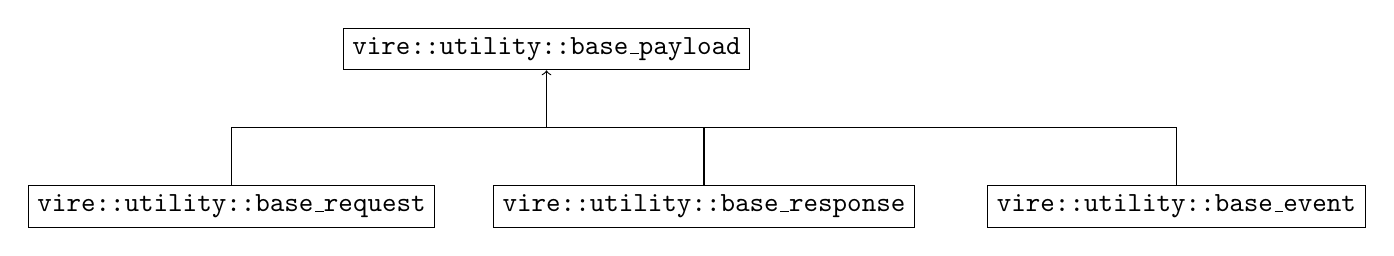
\begin{tikzpicture}
  \node (payload)  at (0,2)  [draw] {\texttt{vire::utility::base\_payload}};
  \node (request)  at (-4,0) [draw] {\texttt{vire::utility::base\_request}};
  \node (response) at (2,0)  [draw] {\texttt{vire::utility::base\_response}};
  \node (event)    at (8,0)  [draw] {\texttt{vire::utility::base\_event}};

  %\draw[style=help lines] (-3,-1) grid (10,4);
  \draw (node cs:name=response,anchor=north) |- (0,1);
  \draw (node cs:name=event,anchor=north)    |- (0,1);
  \draw[->] (node cs:name=request,anchor=north)
  |- (0,1) -| (node cs:name=payload,anchor=south);
\end{tikzpicture}
\end{center}

The requirements for the transmitted object are the following:

\begin{itemize}

\item The  type of the object  must be conventionally associated  to a
  \textit{string identifier}, possibly with a \textit{version number}.
  Each software component  that may send or receive  the object should
  agree on this type identification scheme.

\item For  each software component, the  object type must have  a JSON
  encoding/decoding functions available (whatever programming language
  is used).

\end{itemize}

Vire uses a dedicated format to encode/decode the body of any message.
The structure of  the body contains two kinds  of informations (figure
\ref{fig-app-json-body}):

\begin{enumerate}

\item The \texttt{object\_type\_id} specifies  the type of the encoded
  object  (figure \ref{fig-app-json-type_id}).   This  unique name  is
  conventionaly fixed for a given application. A version tag allows to
  support possible evolution of the object type.

\item The \texttt{object\_serialization\_buffer} is a character string
  that  encapsulated  the  JSON-serialization stream  of  the  encoded
  object.

  \begin{itemize}
  \item Within  the producer  component of  the message,  the encoding
    function associated to the object  type is responsible to generate
    the JSON stream for the object and store it in the buffer.

  \item Within  the consumer  component of  the message,  the decoding
    function associated to the object type is responsible to parse the
    JSON stream stored in the buffer and restore the object in memory.

  \end{itemize}

  It is expected  that, on both sides of the  connection, the software
  components may  access to  dedicated plugins associated  to specific
  object types conventionnaly associated to their type identifiers and
  JSON  encoding/decoding  methods.  The   system  allows  to  support
  modification  in the  structure of  the objects  thansks to  version
  tagging.

\end{enumerate}

\begin{figure}[h]
\vskip 10pt
\small
\begin{Verbatim}[frame=single,xleftmargin=0.cm,label=\fbox{C++}]
struct msg_body {
  type_identifier      object_type_id; // Object type identifier.
  const base_payload * object;         // Handle to a payload object.
};
\end{Verbatim}
\normalsize
\caption{The structure of a message body object (C++).}\label{fig-app-json-body}
\end{figure}

\begin{figure}[h]
\vskip 10pt
\small
\begin{Verbatim}[frame=single,xleftmargin=0.cm,label=\fbox{C++}]
struct type_identifier {
  std::string name;    // Name uniquely identifying the type of object.
  std::string version; // Character string representing the version
                       // of the object type.
};
\end{Verbatim}
\normalsize
\caption{The structure  of the  type identifier  object related  to an
  encoded object (C++).}\label{fig-app-json-type_id}
\end{figure}

Figure \ref{fig-app-json-body-1} shows the formatted body of a
message which encodes a connection request object from the Vire server
to the CMS server.

\begin{figure}[h]
\vskip 10pt
\small
\begin{Verbatim}[frame=single,xleftmargin=0.cm,label=\fbox{\texttt{JSON}}]
{
  "header" : {
     ...
  },
  "body" : {
    "object_type_id" : {
      "name"    : "vire::cmsserver::connection_request",
      "version" : "1.0"
    },
    "object" : {
      ... JSON serialization of the payload object
          of type "vire::cmsserver::connection_request" ...
    }
  }
}
\end{Verbatim}
\normalsize
\caption{Example of  the body of  a JSON formatted message  wrapping a
  payload                object                 of                type
  \texttt{vire::cmsserver::connection\_request},  inherited  from  the
  \texttt{vire::utility::base\_request} type.}
  \label{fig-app-json-body-1}
\end{figure}

\vfill
\pagebreak
\clearpage
